\documentclass[11pt,a4paper]{article}
\usepackage[utf8]{inputenc}
\usepackage[francais]{babel}
\usepackage[T1]{fontenc}
\usepackage[left=2cm,right=2cm,top=2cm,bottom=2cm]{geometry}
\usepackage{graphicx}
\usepackage{url}
\usepackage{hhline}
\usepackage{multicol}

\author{Vincenzo Bazzucchi (249733) et Nicolas Phan Van (239293)}
\title{Rapport de Bonus}
\date{}

\begin{document}
\maketitle

\section{Amélioration graphique: \texttt{BufferedMapDecorator}}
\subsubsection*{Description}
Nous avons décidé de décorer notre carte pour la rendre plus semblable aux cartes topographiques auxquelles nous sommes habitués.
En particulier toute carte possède une légende, une indication de l'échelle et un quadrillage de lignes verticales et horizontales indiquant longitude et latitude. Nous avons été bien attentifs à ce que toutes les composantes dessinées soit calculées en fonction de la taille de l'image, afin que tout soit toujours visible et lisible.
\subsubsection{Mise en œuvre}
Nous avons décidé de déléguer la décoration de la carte à une classe, \texttt{BufferedMapDecorator} qui, malgré son nom, ne constitue pas une application du patron \textit{Decorator}.

Elle fournit deux constructeurs: un permettant de choisir un certain nombre de paramètres et l'autre en demandant moins et utilisant des valeurs par défaut.
Le constructeur se charge d'ajouter un cadre à l'image, dessine le logo EPFL et écrit le titre de la carte, mais surtout il dessine l'indicateur de l'échelle.
La classe fournit en outre une méthode \texttt{addGrid} qui dessine un quadrillage indiquant latitude et longitude. Pour ce faire on demandé à l'utilisateur les points bas gauche et haut droite de la carte, ainsi que sa résolution et le nombre de subdivisions désirées, paramètres nécessaires pour le calcul des dimensions des objets.

La classe possède aussi une méthode \texttt{addLegend} qui dessine la légende de la carte.

Enfin nous proposons une méthode permettant d'écrire l'image en mémoire sur fichier.

\section{Ajout de fonctionnalités}
En écrivant des tests le long du projet, nous nous sommes rendus compte du fait que l'utilisation des cartes OpenStreetMaps et des fichiers HGT permet le dessin de presque n'importe quel endroit sur la planète. Nous avons voulu essayer de généraliser notre code pour qu'il réalise les cartes les plus précises possibles pour toute latitude, longitude et aire données.
\subsection{Éviter les déformations liées à l'utilisation de la projection CH1903: \texttt{Projection}s}
L'utilisation de la projection CH1903 entraîne la déformation de beaucoup de régions en dehors de la Suisse. Nous avons donc ajouté trois classes héritant de \texttt{Projection}:
\begin{enumerate}
    \item \texttt{LambertConformalConicProjection} implémente la projection conique conforme de Lambert, très adaptée au dessin des zones se trouvant aux latitudes moyennes comme les États-Unis, l'Europe et l'Australie. C'est la projection officielle en Belgique et Estonie et de nombreux pays, comme la France, en utilisent une variation \footnote{\url{http://fr.wikipedia.org/wiki/Projection_conique_conforme_de_Lambert}}. Son constructeur a besoin de deux parallèles de référence. Pour la plupart de l'Afrique, de l'Europe, et des États-Unis on peut utiliser les parallèles 20\degre N et 50\degre N. 
    \item \texttt{MercatorProjection} est une projection adaptée dans les régions autour de l'équateur et très utilisée pour la navigation maritime.
    \item \texttt{StereoGraphicProjection} Projection adaptée pour les aires autour des pôles ou pour le dessin de petites cartes continentales.
\end{enumerate}
Les trois projections sont \textit{conformes}\footnote{\url{http://www.icsm.gov.au/mapping/map_projections.html}} c'est-à-dire qu'elles essaient de préserver les formes des objets.

\subsection{Dessin de carte à l'aide de plusieurs fichiers HGT}
L'utilisation d'un seul fichier réduit non seulement le choix de l'aire à dessiner mais aussi celui de la zone (comment faire entre deux fichiers?). Nous avons donc essayé d'implémenter le dessin en utilisant plusieurs fichiers HGT.

\begin{center}
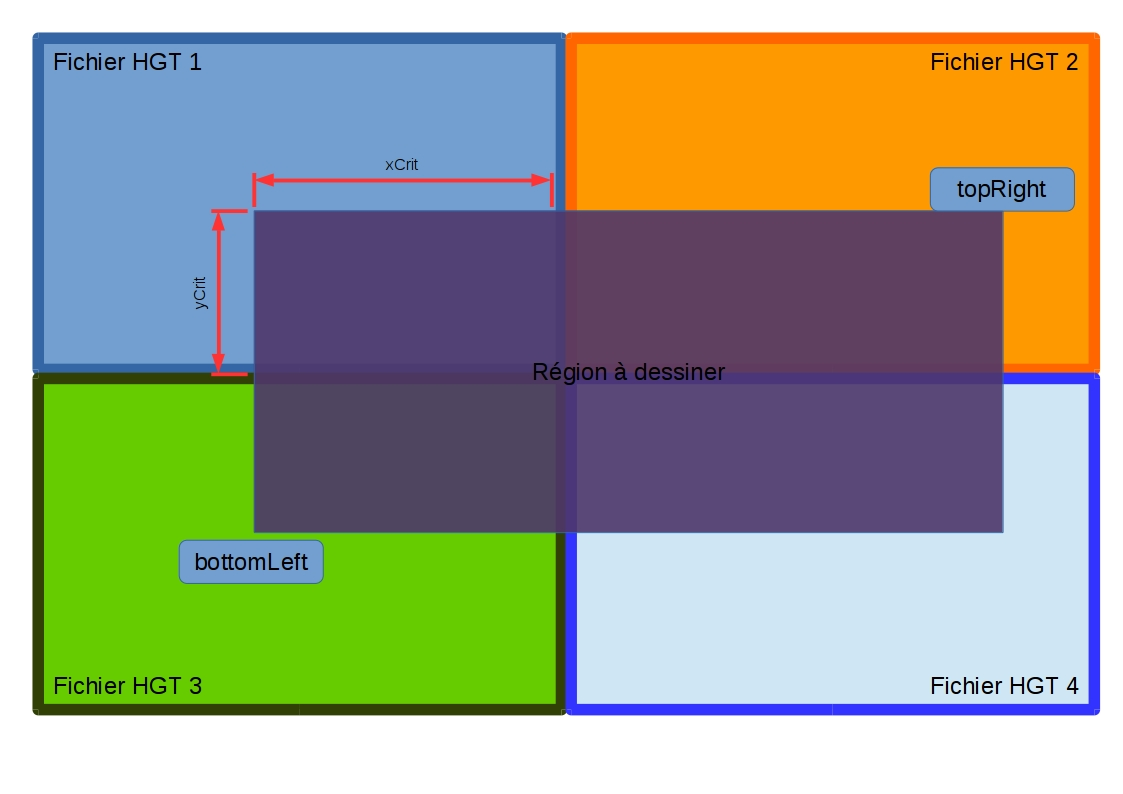
\includegraphics[scale=0.3]{schema4files.jpg}
\end{center}

L'image ci-dessus illustre le cas auquel nous nous sommes intéressés. Arriver à définir le comportement pour le cas de 4 fichiers permet aussi de définir sans difficultés, des méthodes pour dessiner en utilisant 2 fichiers.

\subsubsection*{Mise en œuvre}
Nous avons essayé d'abord d'utiliser les objets \texttt{DigitalElevationModel} définis comme décrit lors de l'étape 11, mais ceci posait un problème de mémoire: instancier plusieurs objets de ce type implique de charger en mémoire tout le contenu du fichier hgt ce qui bloque l'exécution du programme, même en augmentant la quantité de mémoire utilisable par la Machine Virtuelle Java à travers le paramètre \texttt{-Xmx}. Nos tests nous montrent que même avec 8GB la création de 4 objets est impossible.

Nous avons alors décidé de modifier \texttt{DigitalElevationModel} pour fournir une méthode \texttt{loadBuffer()} qui charge en mémoire le contenu du fichier dont la référence est stockée dans l'objet implémentant cette interface. Ceci nous permet de décider quand charger les données en mémoire et quand les retirer de celle-ci à l'aide de la méthode \texttt{close()}.

C'est alors la classe \texttt{ReliefShader} qui s'occupe de gérer les fichiers HGT qu'elle reçoit en fonction de leur nombre. Elle dessine les quatre portions d'images de la carte se trouvant sur les quatre fichiers différents une par une. Pour ce faire nous avons utilisé deux fonctions pour projeter les points du repère de l'image à celui réel et vice-versa afin de pouvoir calculer les distances indiquées par les flèches rouges dans l'image et donc pouvoir choisir le fichier à utiliser et les dimensions de la sous-image à dessiner.

\subsubsection*{Problèmes et inconvénients de cette implémentation}
Malgré nos efforts, nous ne comprenons pas pourquoi le code écrit ne fonctionne pas. Le problème semble naître dans les frontières des fichiers HGT: les hauteurs des points se trouvant à ces coordonnées ne semblent pas êtres contenus dans les fichiers alors qu'ils devraient y être, et en double (une fois sur chaque fichier vu que ceux-ci se chevauchent).

En outre cette solution nous impose de gérer des erreurs d'entrées sorties dans \texttt{ReliefShader} qui n'est qu'une classe de dessin.

Malgré ces aspects nous avons voulu essayer car pouvoir choisir librement la région à dessiner nous semblait important.

\subsection{Téléchargement des fichiers OpenStreetMaps}
Dans la classe \texttt{Main} nous fournissons une petite méthode permettant de télécharger les cartes OSM à travers la \textit{Overpass API}\footnote{\url{http://wiki.openstreetmap.org/wiki/Overpass_API}} conseillée pour le téléchargement de fichiers de grosses dimensions sans impacter les performances de l'API principale de OpenStreetMaps, qui est limitée à des régions carrées de maximum 0.5\degre.
\end{document}
